\documentclass[11pt,a4paper]{article}
\usepackage{amsmath, graphicx, geometry, float}
\usepackage{hyperref, caption, subcaption}
\usepackage{typearea}

\areaset{160mm}{250mm}

\begin{document}
\title{\Large\bf Arbeit zum \\ \textit{Praktikum Mess- und Regelungstechnik} \\ Sommersemester 2022}
\author{Simon Klüpfel, Lukas Zeller \\
  Robotik und Telematik \\
  Universität Würzburg\\
  Am Hubland, D-97074 Würzburg\\
\small \texttt{lukas.zeller@stud.uni-wuerzburg.de} \\
\small \texttt{simon.kluepfel@stud.uni-wuerzburg.de}}
\date{Würzburg, 24.08.2022}

\maketitle

\section{Einleitung zum Volksbot-Roboter}
In dieser Arbeit befassen wir uns mit dem Robot Operating System, kurz \textit{ROS}, und der 
Verwendung dessen auf einem einfachen Roboter, dem \textit{Volksbot}. \\
Der verwendete Roboter ist der \textit{RT3-2} mit zwei passiven Rädern und der \textit{RT-3} mit einem passiven Rad.
Entwickelt wurden diese vom \textit{Fraunhofer Institut IAIS} aus Sankt Augustin. \\
Die technischen Daten sind wie folgt: \\
\vspace{1mm}
\begin{center}
\begin{tabular}{| p{5cm} p{5cm} |}
  \hline
  Abmessungen & 580x520x315mm (L x B x H) \\
  Gewicht & 17kg \\
  
  Raddurchmesser & 260x85mm (aktive Räder) \\
   & 200mm (passive Räder) \\
  Maximale Geschwindigkeit & 2,2 $\frac{m}{s}$ \\
  
  Maximale Zuladung & 25kg \\
  \hline
\end{tabular} \\
\small{ Auszug aus \url{https://www.volksbot.de/rt3-de.php}}
\end{center}
\vspace{5mm}
Auf dem Roboter ist ein Laserscanner sowie Hardware zur Verbindung mit dem verwendeten
Laptop installiert. Außerdem lässt sich der Roboter über einen Joystick, ähnlich eines Gamecontrollers, manuell steuern. 
Wir verwenden sowohl vorgegebene ROS-Nodes, die uns von Institut für Robotik und Telematik zur Verfügung gestellt wurden, als auch angepasste Nodes die wir selbst erstellt beziehungsweise
geändert haben. 
\vspace{5mm}
\begin{figure}[H]
  \caption*{Abbildung 1: Volksbot RT3 und Logitech G710-Gamecontroller}
  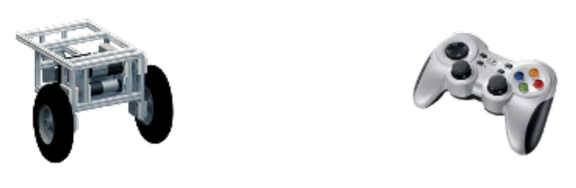
\includegraphics[]{robotandcontroller.pdf}
  \centering
\end{figure}
\newpage

\section{Kartierung mit GMapping}
Wir starten zuerst die Node zur Kommunikation mit dem Roboter: \begin{verbatim}
  roslaunch volksbot messtechnikpraktikum.launch
\end{verbatim}
Um den Roboter zu steuern mit dem Controller benötigen wir die zugehörige Node: \begin{verbatim}
  roslaunch volksbot localjoystick.launch
\end{verbatim}
Nun erstellen wir eine \textit{rosbag}, die alle Topics des Roboters aufzeichnet: \begin{verbatim}
  rosbag record -a
\end{verbatim}
Um nun eine Karte erstellen zu können, müssen wir die aufgenommene \textit{bag} abspielen. 
Wichtig hier ist es den Parameter \begin{verbatim}
  rosparam set use_sim_time true
\end{verbatim} zu setzen um die Zeit aus dem \textit{clock}-Topic zu nutzen anstelle der globalen Systemzeit.
Nun kann man aus den Laserscanner-Daten, also hauptsächlich dem \textit{LMS}-Topic, die Map
erstellen. Hierzu starten wir das GMapping-Tool via \begin{verbatim}
  roslaunch volksbot messtechnikgmapping.launch
\end{verbatim}
Die Bag kann dann abgespielt werden mit \begin{verbatim}
  rosbag play filename.bag --clock
\end{verbatim}
Der \textit{clock}-Befehl am Ende ist wichtig um die Aufnahmen der \textit{rosbag} mit einem 
Zeitstempel zu versehen damit der Roboter sie nicht verwirft. 
Startet man nun RViz kann man über das \textit{map}-Topic den Aufbau der Map betrachten.
Um diese zu speichern startet man eine \textit{ROS-node} die das \textit{map}-Topic in
eine Datei speichert. 

\begin{figure}[H]
  \caption*{Abbildung 2: Aufgezeichnete Karte des Informatik-Untergeschosses}
  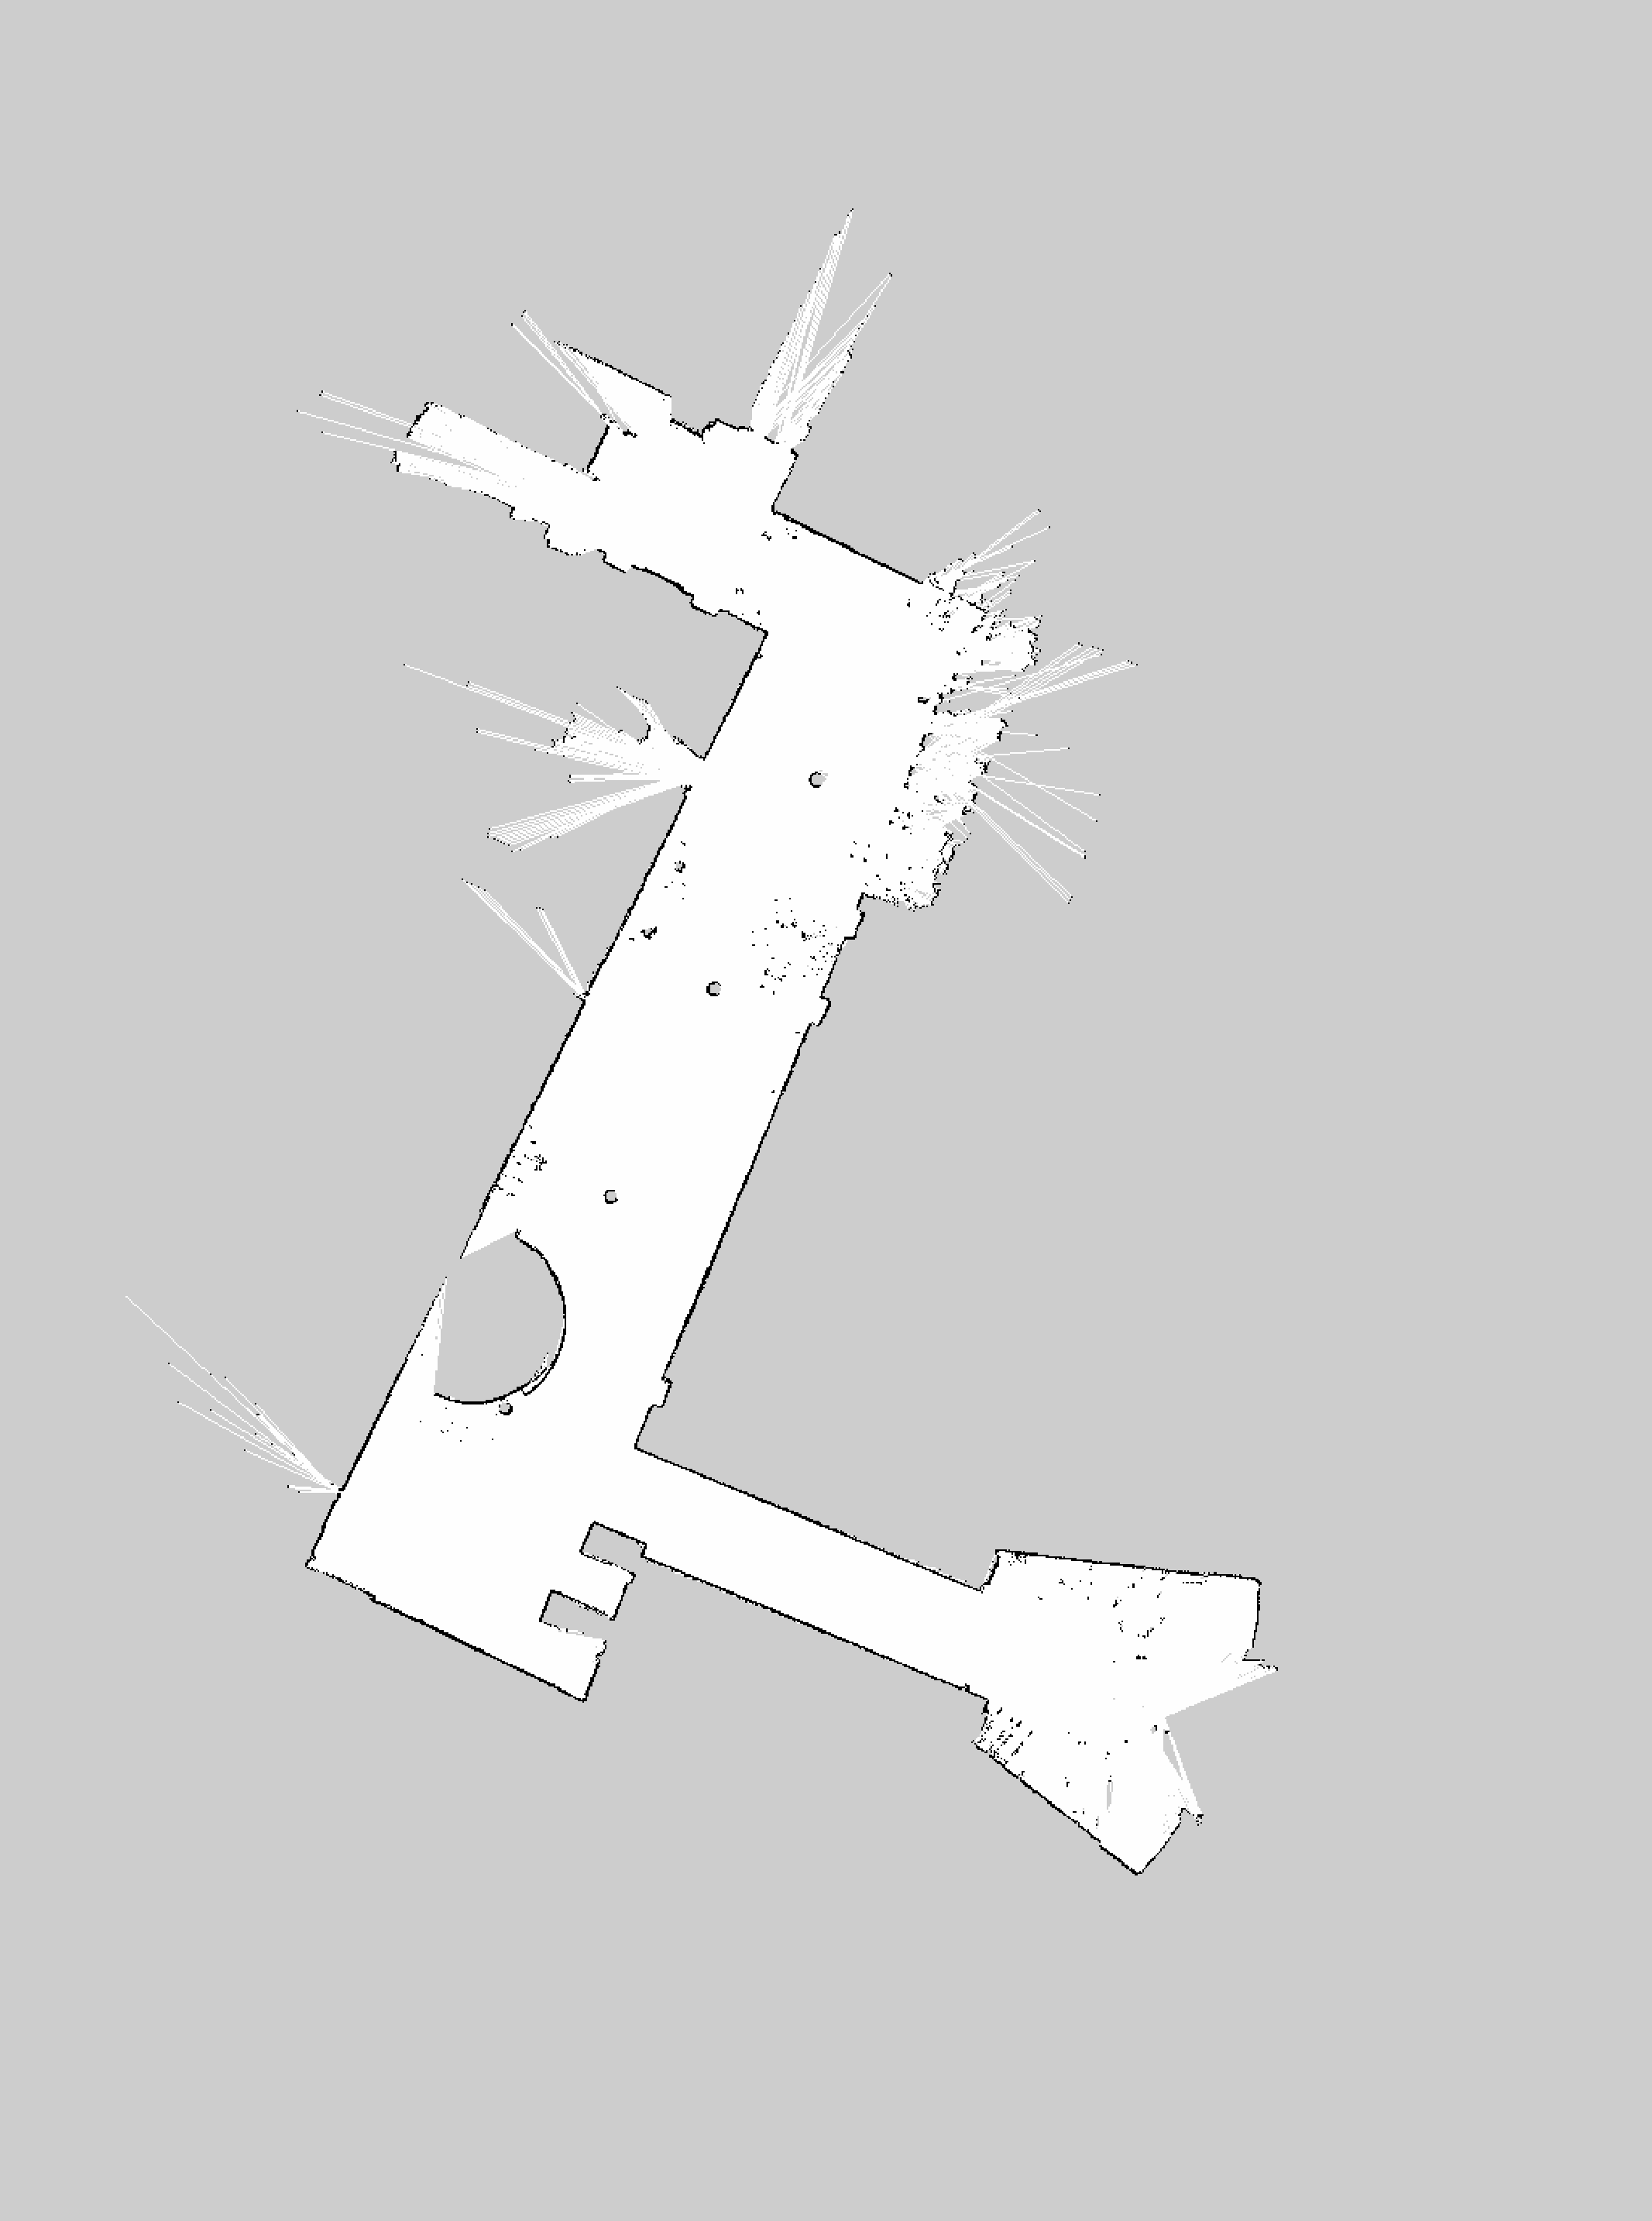
\includegraphics[scale = 0.3, angle = 90]{map.pdf}
  \centering
\end{figure}

% KOM: das ist falsch. zuerst fahren wir daten in eine Bag und machen aus der bag ne map
% KOM: wir brauchen dazu keine plots??? Wir haben nicht mal relevante. Ein bild der karte die wir rausbekommen haben reicht

\section{AMCL-Lokalisierung}
Um aus der Odometrie einen Pfad zu plotten erstellen wir ein eigenes ROS-Node. Das Node-Package heißt \verb|data_saver|, 
die Node an sich \texttt{listener}. Es ist Subscriber des Odometrie-Topics und speichert die empfangenen Daten 
in einer Datei im Format \verb|Xpos_Ypos| \\
Es hat zwei Modi, wie es diese Daten speichern kann:
\begin{center}
\texttt{rel}: Koordinaten im Pfad sind relativ zum Roboter \\
\texttt{abs}: Koordinaten sind absolut aus dem AMCL-Frame \\
\end{center}
Man starte sie mit dem gewählten Modus:
\begin{verbatim}
  rosrun data_saver listener_mode := "abs || rel"
\end{verbatim}
Um AMCL zu starten nutzen wir die vorgegebene Launchfile:
\begin{verbatim}
roslaunch volksbot messtechnikamcl.launch
\end{verbatim}
Bei Betrachten des launchfile-Codes fällt auf dass zusammen mit dem AMCL-Node ein \verb|map_server|-Node gestartet
wird, welches eine vorgegebene Map published. Wir wollen aber unsere eigene Map verwenden, weswegen wir diese Zeile
auskommentieren und stattdessen eine eigene \verb|map_server|-Node starten, welches die Map aus \textit{GMapping}
published: \begin{verbatim}
rosrun map_server map_server map.yaml
\end{verbatim}
Außerdem muss im Configuration-File von AMCL noch eingefügt werden, dass AMCL auf ein Map-Topic subscriben soll,
und wie dieses Topic heißen soll. \\
In RViz muss man nun noch die Position des Roboters festlegen. Dazu setzt man die Map und das \verb|amcl_pose|-Topic
sichtbar, in unserem Fall mittels einer .config-File, die man über \begin{verbatim}
rviz -d config.rviz
\end{verbatim}
ausführt.
In RViz drückt man nun den \verb|2D-Pose-Estimate|-Button, dann an die Stelle der Karte wo der Roboter am Anfang steht,
hält dabei gedrückt, und bewegt die Maus in die Richtung in die die Roboterlängsachse zeigt. Zum Bestätigen
lässt man den Mausbutton los. \\
Um die \texttt{rosbag}-Datei nun abspielen zu können, führe man folgenden Befehl im Terminal aus:
\begin{verbatim}
rosbag play file.bag --clock
\end{verbatim}
Der Roboter bewegt sich nun in RViz virtuell auf der Karte und lokalisiert sich dabei mit AMCL.

\begin{figure}[H]
  \caption*{Abbildung 3: RViz-Screenshot: Roboter lokalisiert sich in der Karte mittels AMCL}
  \includegraphics[scale = 0.25]{amcllocalisation.png}
  \centering
\end{figure}

\section{Pfadverfolgung}
% KOM: du musst auf die Koordinatensysteme von AMCL/Odom eingehen. Das ist das Hauptthema im Code.

% KOM: du musst auf die Koordinatensysteme von AMCL/Odom eingehen. Das ist das Hauptthema im Code.

\section{Auswertung}
todo: 
Testen Sie den Regler mit dem aufgenommenen Pfad aus dem Informatikgebäude. Vergleichen Sie das Verhalten, wenn einmal die Odometrie und einmal die von AMCL bestimmten
Positionen als Messwerte für die Regelung verwendet werden.

also: plots, kommentare, was ist besser, was schlechter?

% KOM: An Plots brauchen wir hier Simulation, den rohen Pfad, AMCL, Odom, und Bilder was er IRL jeweils getan hat. Die Bilder kann ich noch machen.



\end{document}

